
%(BEGIN_QUESTION)
% Copyright 2011, Tony R. Kuphaldt, released under the Creative Commons Attribution License (v 1.0)
% This means you may do almost anything with this work of mine, so long as you give me proper credit

Read selected portions of the Allen-Bradley ``Logix5000 Controllers General Instructions'' reference manual (publication 1756-RM0031-EN-P, January 2007) and answer the following questions:

\vskip 10pt

Identify the different types of {\it counter} instructions offered in the Logix5000 PLC family.

\vskip 10pt

How high can one of these counter instructions count up to?  How low can it count down to?  Based on these values, how many bits do you think are used in the register to store a counter instruction's current value?

\vskip 10pt

Unlike the Siemens S7 family of PLCs, the Allen-Bradley counter instruction ``box'' symbols do not provide a  place to connect a {\it reset} input.   How then is it possible to command a counter instruction to reset back to zero?

\vskip 10pt

Sketch a simple ladder-diagram program for an Allen-Bradley Logix5000 PLC whereby a high-temperature switch input with the tag-name {\tt High\_Motor\_Temp} causes a counter to increment (count {\it up}) every time a motor overheats, and then turn on an alarm light output (tag-name {\tt Alarm\_Lamp}) when the count reaches a value of 5.  Also provide a ``reset'' function triggered by a normally-open switch contact (tag-name {\tt Alarm\_Reset}) to force the count value back to zero when pressed.


\vskip 20pt \vbox{\hrule \hbox{\strut \vrule{} {\bf Suggestions for Socratic discussion} \vrule} \hrule}

\begin{itemize}
\item{} If you have access to your own PLC for experimentation, I urge you to write a simple {\it demonstration} program in your PLC allowing you to explore the behavior of these PLC instructions.  The program doesn't have to do anything useful, but merely demonstrate what each instruction does.  First, read the appropriate section in your PLC's manual or instruction reference to identify the proper syntax for that instruction (e.g. which types of data it uses, what address ranges are appropriate), then write the simplest program you can think of to demonstrate that function in isolation.  Download this program to your PLC, then run it and observe how it functions ``live'' by noting the color highlighting in your editing program's display and/or the numerical values manipulated by each instruction.  After ``playing'' with your demonstration program and observing its behavior, write comments for each rung of your program explaining in your own words what each instruction does.
\end{itemize}

\underbar{file i02664}
%(END_QUESTION)





%(BEGIN_ANSWER)


%(END_ANSWER)





%(BEGIN_NOTES)

Three types of counter instructions: count up (CTU), count down (CTD), and count up/down (CTUD).  CTU and CTD are the only types of counter instructions available in ladder logic, though -- the CTUD instruction is strictly used in {\it function block} programming.

\vskip 10pt

Each of the Logix5000 counter instructions can count as high as +2,147,483,647 and as low as $-2,147,483,648$.  This equates to 32 bits, signed integer (2's complement notation, where the MSB has a negative place-weight value of $-2,147,483,648$).

\vskip 10pt

Logix5000 counter instructions are reset by the use of a special ``Reset'' coil instruction, addressed to that counter.

\vskip 10pt

Simple counter program to fulfill stated requirements:

$$\includegraphics[width=15.5cm]{i02664x01.eps}$$

%INDEX% Reading assignment: Allen-Bradley Logix5000 instruction reference manual (counter instructions)

%(END_NOTES)


